
\begin{section}{Approach}
\label{sec:approach}

\NB{add text here to introduce what the reader will see in the next few sections. Add a block diagram}

% INSERT FIGURE FOR THE ARCHITECTURE OF THE SYSTEM HERE
%\begin{figure}[ht!]
%	\centering
%	\includegraphics[width=0.48\textwidth]{det_arch.png}
%	\caption{Architecture of our adaptive system to include detection capabilities}
%	\label{fig:det_arch}
%\end{figure}

\begin{figure}
\vspace{1pt}
\centering
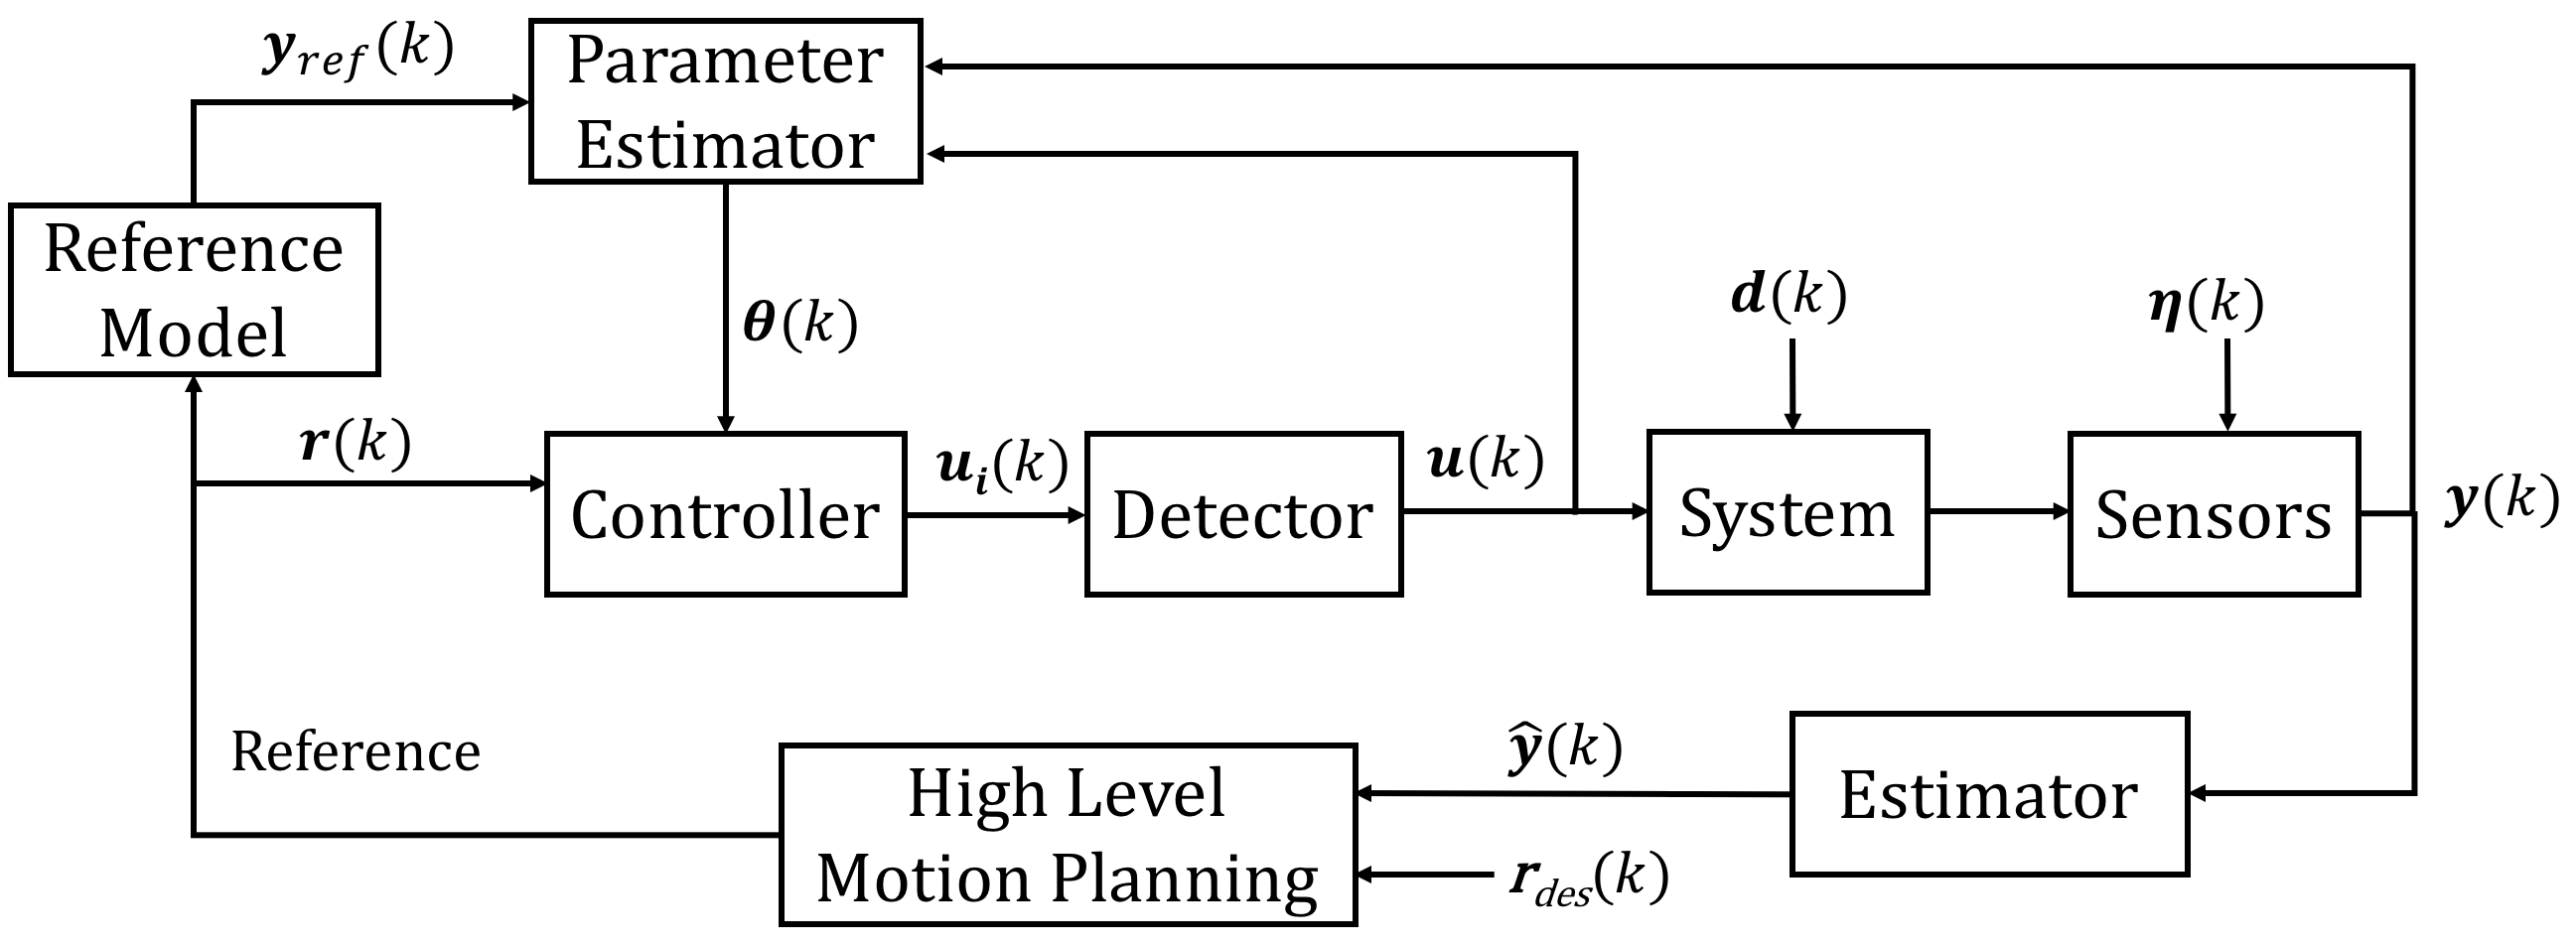
\includegraphics[width=0.48\textwidth]{sys_arch.png}
\caption{Overall system architecture showing the relationship between the reference model adaptive controller and the adaptive motion planner.}
\label{fig:system_arch}
\end{figure}

\subsection{Model Reference Adaptive Control}

\NB{merge section A and B and titled it Resilient Adaptive Control. Summarize more what in section A and shift teh attention to the detection and estimation}
The purpose of having a model reference adaptive controller is to maintain a desired control performance when unknown dynamical changes or disturbances have occurred. Estimation of the system's polynomial coefficients will help give us this desired performance.
Assumptions for adaptive control: 
	\begin{enumerate}[leftmargin=4\parindent]
	\item[$A1)$] all zeros of $B^{'}(z^{-1})z^m$ are within $|z|<1$. 
	\item[$A2)$] $n$ and $m$ (or their upper bounds) are known. 
	\item[$A3)$] the system delay $d$ is known.
	\end{enumerate}
The objective of model reference adaptive control is to calculate an input signal $u(k)$ such that the system tracks $y^{*}(k)$ given the reference signal $r(k)$. 
A following assumption for the reference model is it satisfies:
    \begin{enumerate}[leftmargin=4\parindent]
	\item[$A4)$] all zeros of $E(z^{-1})z^p$ are within $|z|<1$. 
	\end{enumerate}

The model reference control is designed (Reference to equation!) by solving the polynomial equation:
    \begin{equation}
	E(q^{-1})=F(q^{-1})A(q^{-1})+q^{-d}G(q^{-1})
	\end{equation}
By expressing (Ref to equation $A(q^{-1})y(k)=B(q^{-1})u(k)$) as:
	\begin{equation}
	E(q^{-1})y(k+d)={\alpha}q^{-1}y(k) + {\beta}q^{-1}u(k)=\theta_0^T\phi(k)
	\end{equation}
where,
	\begin{equation}
	\alpha(q^{-1})=G(q^{-1})=\alpha_0+\alpha_1q^{-1}+ \dots +\alpha_{n-1}q^{-n+1}
	\end{equation}
	\begin{align}
	\beta( & q^{-1})=F(q^{-1})B^{'}(q^{-1})=\beta_0+\beta_1q^{-1} \nonumber \\
	& + \dots +\beta_{m+d-1}q^{-m-d+1}, \beta_0\neq0
	\end{align}
we are designing the system to have the same characteristics as the reference model. Parametrization to express this system is:
	\begin{equation}
	\bm{\theta}_0=(\alpha_0, \dots ,\alpha_{n-1},\beta_0, \dots ,\beta_{m+d-1})^T \in R^{n+m+d}
	\end{equation}
	\begin{align}
	\bm{\phi}(j)&=(y(k), \dots ,y(k-n+1),u(k), \dots , \nonumber \\
	& u(k-m-d+1))^T \in R^{n+m+d}
	\end{align}
where $\bm{\theta}_0$ is unknown and $\bm{\phi}(k)$ is known.
	The adaptive control input u(k) is then calculated from the equation:
	\begin{equation}
	\bm{\theta}^T(k)\bm{\phi}(k)=E(q^{-1})y^{*}(k+d)
	\end{equation}
with the equation for the input u(k) as:
	\begin{align}
	u(k)=\frac{1}{\theta_{n+1}(k)}&(-\theta_1(k)y(k)-\theta_2(k)y(k-1)  \nonumber \\
    -\dots-\theta_n(k)y(k&-n-1)-\theta_{n+2}(k)u(k-1)  \\
	-\theta_{n+3}(k)u(k-2)-& \dots - \theta_{n+m+d}(k)u(k-m-d+1) \nonumber \\
	+g&H(q^{-1})r(k))^T \nonumber
	\end{align}
	\begin{equation}
	\bm{\theta}(k)=(\theta_1(k), \dots ,\theta_n(k),\theta_{n+1}(k), \dots ,\theta_{n+m+d}(k))^T
	\end{equation}
where $\bm{\theta}(k)$ is the estimate of the true parameter vector $\bm{\theta}_0$, updated by the modified projection algorithm:
	\begin{equation}
	\bm{\theta}(k)=\bm{\theta}(k-1)+\frac{a(k)\phi(k-d)e(k)}{c+\phi^T(k-d)\phi(k-d)}
	\end{equation}
	\begin{equation}
	\bm{e}(k)=E(q^{-1})y(k)-\theta^T(k-1)\phi(k-d)
	\end{equation}
	\begin{align*}
	\varepsilon<a(k)<2-\varepsilon, 0,\varepsilon<1, c>0
	\end{align*}
To avoid division by $0$, $\theta_{n+1}(k)\neq0$ is necessary.

\subsection{Detection}

For detection, model reference adaptive control is an effective solution to the problem of dynamically changing or unknown systems. From (CITE reference) states that under the assumptions (reference to all 4 assumptions) ensures:
	\begin{enumerate}[label=(\roman*),leftmargin=4\parindent]
	\item $y(k)$ and $u(k)$ are bounded 
	\item $\lim_{n\to\infty}(y(k)-y^*(k))=0$
	\item $\sum_{k=0}^\infty(y(k)-y^*(k))^2<\infty$
	\end{enumerate}
	
	\begin{figure}[ht!]
\vspace{1pt}
\centering
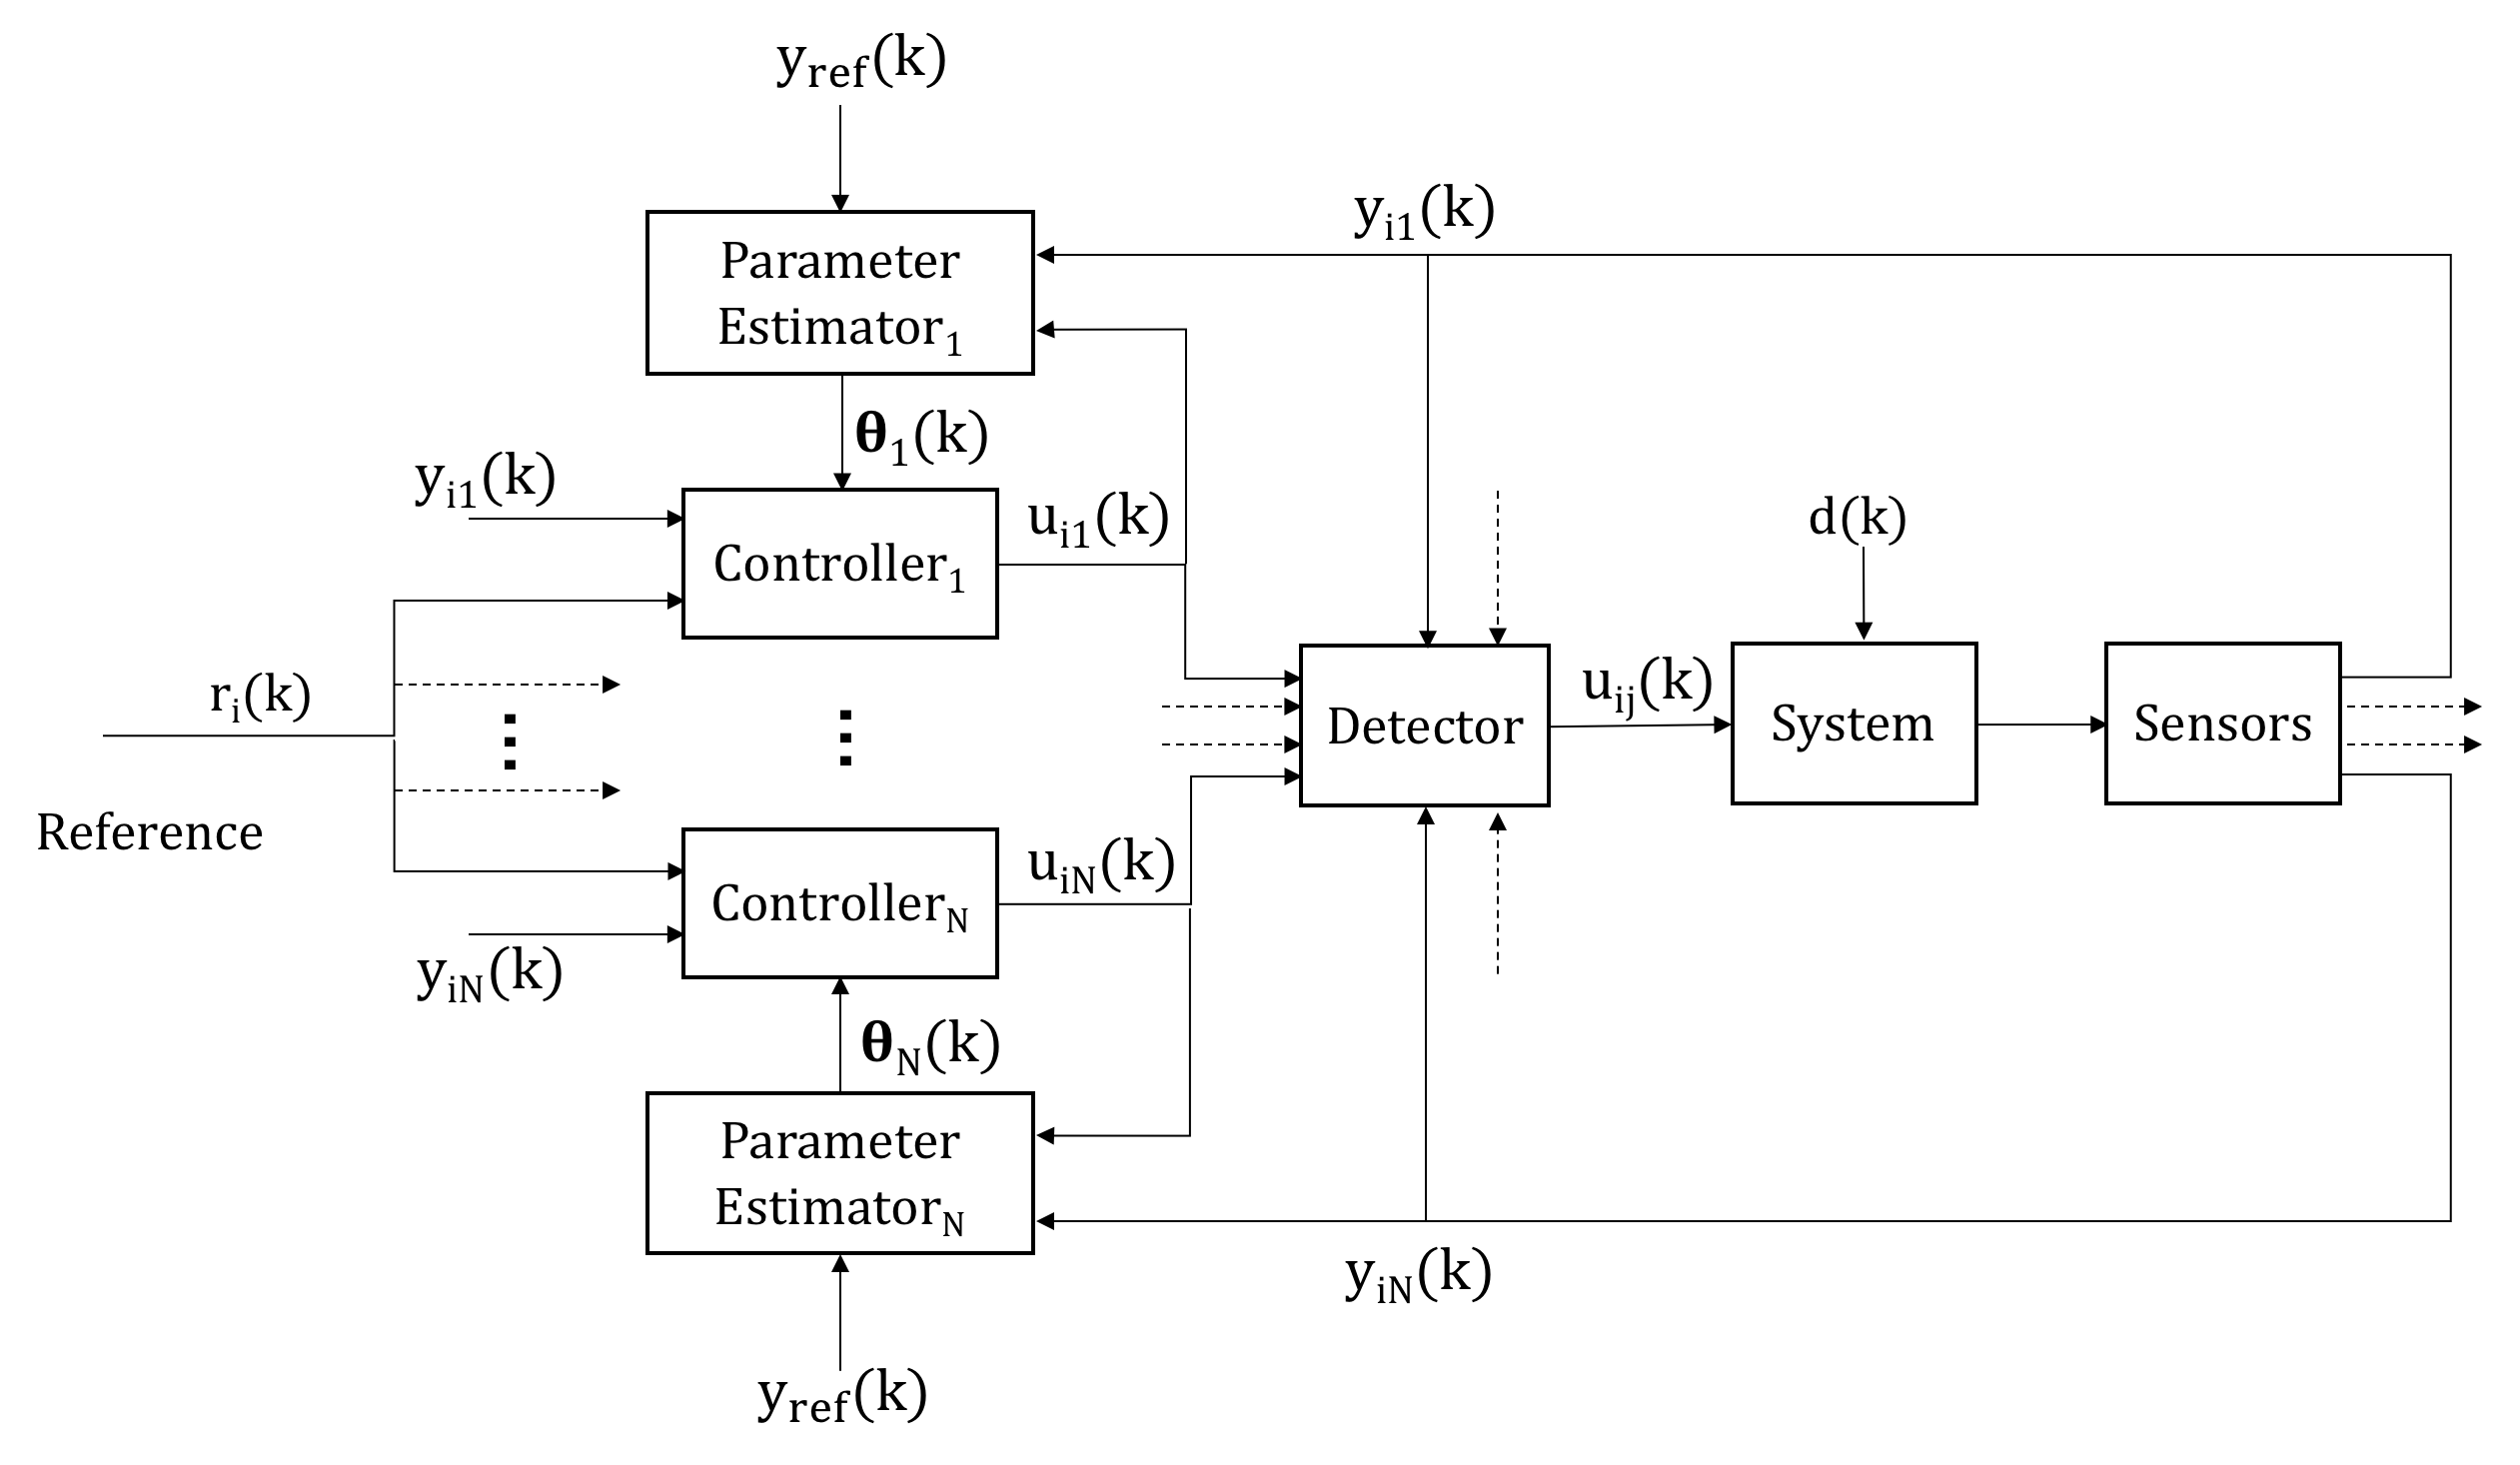
\includegraphics[width=0.48\textwidth]{con_and_det.png}
\caption{System architecture of the detection scheme within the adaptive controller. Representing the $i^{th}$ state and the $j$ number of available sensors.}
\label{fig:det_arch}
\end{figure}

\NB{equations and symbols in the figures should look like the text}

This states the system's output $y(k)$ will asymptotically converge to the tracking reference signal $r(k)$ in a finite amount of time. Properties of the modified projection algorithm include,
    \begin{enumerate}[label=(\roman*),leftmargin=3\parindent]
	\item every iteration improves estimation:
	    \begin{align}
	        \|\bm{\theta}(k)-\bm{\theta}_0\|\leq\|\bm{\theta}(k-1)-\bm{\theta}_0\|\leq\|\bm{\theta}(0)-\bm{\theta}_0\|, k\geq1 \nonumber
	    \end{align}
	\item parameter variation has finite energy:
	    \begin{align}
	        \sum_{k=1}^\infty{\|\bm{\theta}(k)-\bm{\theta}(k-1)\|}^2\leq \infty \nonumber
	    \end{align}
	\item parameter variation converges to zero:
	    \begin{align}
	        \lim_{k\to\infty}(\bm{\theta}(k)-\bm{\theta}(k-1))=0 \nonumber
	    \end{align}
	    \begin{align}
	        \lim_{k\to\infty}(\bm{\theta}(k)-\bm{\theta}(k-N))=0, \text{any finite } N>0 \nonumber
	    \end{align}
	\end{enumerate}

Each system state $\bm{x}_i$ where $i=1,2,\dots,n_x$ and $n_x$ is the total number of states has sensors $\bm{s}_{ij}$ for $j=1,2,\dots,n_{s_i}$ where $n_{s_i}$ is the number of sensors that can extract sensor measurement data for a given state. These sensor measurements adhere to the above adaptive control assurances, with the addition of noise uncertainties.

Each of the sensors $\bm{s}_{ij}$ providing measurement data of each states experience the same convergence behavior to the tracking signal where sensors are uncompromised. This remains true with a changing reference signal, system dynamics, or bounded disturbances. When an attacker maliciously falsifies a sensor signal, the $j^{th}$ sensor of the $i^{th}$ state from the sensor set $\bm{s}_{ij}$ no longer follows the converge rate compared to the uncompromised sensor measurements. 
\NB{add missing equations}
\NB{add Lemma}

\subsection{Sensor Removal}

\NB{be careful with the indexes. $n$ states and $i,j,k$ are indeces}

As the $j^{th}$ sensor of the $i^{th}$ state no longer follows convergence characteristics, it is removed from operation to ensure proper control and navigation safety. The new set of sensors providing measurement data for the $i^{th}$ state is $\bm{s}_{ij}^*$ where $j^*=1,2,\dots,n_{s_i}-h_s$ \NB{$y$ for measurements} when $h_s$ is defined as the total number of compromised sensors.

\subsection{Estimation}

\NB{Say what's happening here and why} The statistical technique of confidence intervals is the foundation of how this work solves estimation. Confidence intervals are used to estimate the mean of a population of data in stochastic environments. \NB{show equation here} This method guarantees the true mean has a specific percentage of confidence that it's within an interval. Assuming the knowledge of the confidence percentage $z^{*}$, sensor noise standard deviation $ \sigma_p $, the number of sensor data samples $N$, and the mean of the sensor data samples $ \bm{\bar{x}}_{x,y} $ in the $x$ and $y$ direction, a confidence interval of a chosen percentage can be calculated \NB{define $\epsilon$}: 
 	\begin{equation}
		\varepsilon_{x,y|N} = \bar{s}_{x,y} + z^{*}\frac{\sigma}{\sqrt{N}}
	\end{equation}
This is under the assumption that the true mean is not changing over the previous $N$ number of sampled data points used in the current confidence interval calculation.

Assuming the data being used for estimation, regardless if it's raw or filtered data, is that it comes in the form $\mathcal{N}(0,\sigma_d)$ where the data population standard deviation $\sigma_d$ is known for any sensor combination. From [reference to above equation] we can find an interval of a determined confidence percentage that the vehicle is within that region to ensure safety. 

The assumption of a confidence interval is the true mean remains static on the given axis. This cannot be assumed in the case of position estimation of a navigating vehicle. A pseudo-static form of a confidence interval is made to compensate for translation of position $\bm{x}(k-M)$, where $M=1,2,\dots,N-1$. The $M$ number of previous position data points are represented as if they all were taken from the current position $\bm{x}(k)$ in time. (SHOW THIS IN A FIGURE FOR BETTER VISUAL UNDERSTANDING, either Matlab or Powerpoint). These samples $\bm{x}_p$, where $p=1,2,\dots,N$ form the set $\mathcal{\bm{S}}=\begin{bmatrix}\bm{x}_1,\bm{x}_2,\dots,\bm{x}_N \end{bmatrix}$. Further, we can break down the set into two vectors $\bm{s}_x=\begin{bmatrix} x_{x1},x_{x2},\dots,x_{xN} \end{bmatrix}$ and $\bm{s}_y=\begin{bmatrix} x_{y1},x_{y2},\dots,x_{yN} \end{bmatrix}$ which represent the $x$ and $y$ coordinate data, respectively. 

Translating the data coordinates into a pseudo-static form will create the set $\mathcal{\bm{S}}_t$, creating the two pseudo-static vectors $\bm{s}_{t_x}=\begin{bmatrix} x_{t_{x1}},x_{t_{x2}},\dots,x_{t_{xN}} \end{bmatrix}$ and $\bm{s}_{t_y}=\begin{bmatrix} x_{t_{y1}},x_{t_{y2}},\dots,\bm{x}_{t_{yN}} \end{bmatrix}$. Each element of these updated vectors are calculated as:
    \begin{equation}
	x_{t_{xw}} = x_x(k-w+1)+\sum_{j=1}^w v(k-j)\cos{\theta_h(k-j)T_s}
	\end{equation}
	\begin{equation}
	x_{t_{yw}} = x_y(k-w+1)+\sum_{j=1}^w v(k-j)\sin{\theta_h(k-j)T_s}
	\end{equation}
The mean of each vector is written as $\bar{s}_x$ and $\bar{s}_y$ is used for the calculation of the confidence interval.

Creating a pseudo-static case with these past position data samples introduces higher uncertainty. Uncertainties regarding the actuator $\sigma_a$, current velocity sensor $\sigma_v$, and current heading angle sensor $\sigma_h$ need to be accounted for. To guarantee the true position of the vehicle is within the estimation radial bounds $\epsilon$, the maximum error in position due to the actuator and sensor noises over the furthest sample in time in $\mathcal{\bm{S}}$ is calculated as:
    \begin{equation}
	\varepsilon_{v,\theta_h|(M)}^{\star}=\sqrt{(v^{\star}\cos{\theta_h^{\star}})^2+(v^{\star}\sin{\theta_h^{\star}})^2}
	\end{equation}
where,
    \begin{equation}
	v^{\star}=\bar{v}(k-i_{\varepsilon^{\star}})+z^{*}\sigma_v \nonumber
	\end{equation}
	\begin{equation}
	\theta_h^{\star}=\bar{\theta}_h(k-i_{\varepsilon^{\star}})+z^{*}\sigma_h \nonumber
	\end{equation}
with $i_{\varepsilon^{\star}}=[1,M]$ while measured velocity and heading angles are denoted $v$ and $\theta_h$, respectively. Doing this will protect the integrity of the confidence interval percentage, ensuring the vehicle is within the estimation bounds.

\subsection{Adaptive Motion Planning}
With uncertainty of sensor measurements, with or without the loss of a compromised sensors, there needs to be guarantees to safely navigate a vehicle without accidents. As obstacles or unwanted regions approach the vehicle with position uncertainty, changes to the vehicle's motion need to be made. To keep the vehicles estimated confidence region from intersecting with an unwanted region, a change to the number of current and past data samples in the calculation as well as an adaptation of the velocity. With no uncertainty of velocity and heading angle measurements, the equation to solve for the number of required $N$ samples to keep the confidence interval within a specific radius is:
    \begin{equation}
	    N_{k+1} \geq \left(z^{*} \frac{ \sigma_p }{ {\lVert \bm{x}_{r_{\bar{s}}} - \bar{s}_{x,y} \rVert} -\Delta(k) } \right)^2
	\end{equation}
where $\lVert {\bm{x}_{r_{\bar{s}}}-\bar{s}_{x,y}} \rVert$ is the distance from the closest undesired region to the estimated position mean $\bar{s}_{x,y}$.
With the assumption of Normally distributed sensor noise on the velocity and heading angle sensors, the above equation is not suitable. The uncertainty region $\varepsilon_{v,\theta_h|(M)}^{\star}$ from these sensors must be accounted for. The revision to equation (Equation above) for a sufficient value of $N$ is:
    \begin{equation}
	    N_{k+1} \geq \left(z^{*} \frac{ \sigma_p }{ {\lVert \bm{x}_{r_{\bar{s}}} - \bar{s}_{x,y} \rVert} -[\varepsilon_{v,\theta_h|(M_k)}^{\star}+\Delta(k)] } \right)^2
	\end{equation}
An update of the reference velocity needs to occur when these undesired regions are within the entire confidence estimation region $ \varepsilon_{x,y|N} +\varepsilon_{v,\theta_h|(N-1)}^{\star}+\Delta(k)$ when $N=1$ to ensure the vehicle slows to capture more previous data samples with less estimation error. This reference velocity $r_v$ update is calculated by,
    \begin{equation}
	    r_v(k)=r_v(k-1) \left[ \frac{\lVert \bm{x}_{r_{\bar{s}}} - \bar{s}_{x,y} \rVert - \varepsilon_1}{\varepsilon_2 - \varepsilon_1} \right]
	\end{equation}
	\begin{equation}
	\begin{split}
	    \varepsilon_1=&\varepsilon_{x,y|N_k} +\varepsilon_{v,\theta_h|(M_k)}^{\star},\\ &\varepsilon_2=\varepsilon_1+\Delta(k) \nonumber	    
	\end{split}
	\end{equation}


% INSERT ALGORITHM FOR REPLANNING VELOCITY
\begin{algorithm}
   \caption{Adaptive Motion for Safe Navigation} 
   \label{alg:adapt_motion} 
    \begin{algorithmic}[1]
	\State Initial conditions of system: $k=0$,$\bm{x}(0)=\bm{x}_0$
	\State Set $r_v(0)$ to desired velocity $r_{v_{des}}(k)$
    \While{$1<k\leq\infty$}
        \State \Longunderstack[l]{ Measure closest distance to undesired \\ region $\|\bm{x}_{r_{\bar{s}}} - \bar{s}_{x,y}\|$}
        \State Calculate intervals $\varepsilon_1$, $\varepsilon_2$, and $\Delta(k)$ for $N$
        \If{ $\|\bm{x}_{r_{\bar{s}}} - \bar{s}_{x,y}\| < \varepsilon_2(k)$}
            \State Solve for suitable $N_{k+1}$
            \State Update reference for velocity $r_v(k)$
        \Else
            \If{$\|\bm{x}_{r_{\bar{s}}} - \bar{s}_{x,y}\| < \varepsilon_2(k)$ when $N=1$}
                \State Solve for a suitable $N_{k+1}$
                \State Update reference for velocity $r_v(k)$
            \Else
                \If{$r_v(k) \neq r_{v_{des}}$}
                    \State Reference velocity $r_v(k)=r_{v_{des}}$
                    \State $N_{k+1} = 1$
                \Else
                    \State Reference velocity $r_v(k) = r_v(k-1)$
                    \State $N_{k+1} = 1$
                \EndIf
            \EndIf
        \EndIf
        \State $N = N_{k+1}$
    \EndWhile
	\end{algorithmic}
\end{algorithm}



\end{section} 